\documentclass{beamer}

\usepackage[utf8]{inputenc}
\usepackage[spanish]{babel}
\usepackage{tikz}
\usepackage{booktabs}
\usepackage{pgfplots}
\usepackage{subfigure}
% \usepackage{titling} % adds \theauthor \thetitle etc
\usepgfplotslibrary{dateplot}

\newcommand{\titulo}{Python para el cálculo científico}
\newcommand{\autor}{Daniel Lubián Arenillas}
\newcommand{\fecha}{12 de febrero de 2018}
\newcommand{\git}{\texttt{git}}

\title{\titulo}
% \subtitle{¿Cómo usarlo?}
\author{\autor}
%\institute[IDR/UPM]{IDR/UPM}
\date{\fecha}
% \logo{
\includegraphics[height=1cm]{fig/git_logo.eps}}

\usepackage{listings}
\usepackage{verbatim}

% \usetheme{Rochester}
\usetheme{metropolis}
\metroset{block=fill, numbering=fraction, sectionpage=progressbar}%,subsectionpage=progressbar}%,titleformat=smallcaps}
% \usecolortheme{structure}

% \setbeamertemplate{frame footer}{\autor\,--\,\titulo}
% \definecolor{azuletsiae}{RGB}{59,80,141}
% \definecolor{azulclaroetsiae}{RGB}{197,208,228}
% \definecolor{black1}{RGB}{26,28,34}
% \setbeamercolor{normal text}{fg=black1}
% \setbeamercolor{frametitle}{bg=azuletsiae}
% % \setbeamercolor{frametitle}{bg=black1}
% \setbeamercolor{progress bar}{fg=black1}
% \setbeamercolor{progress bar}{fg=azuletsiae,bg=white}
% \setbeamercolor{progress bar}{fg=azuletsiae,bg=azulclaroetsiae}
\titlegraphic{
	% 
\includegraphics[height=1cm]{fig/git_logo_name.eps}
	\hfill
	
\includegraphics[height=1.5cm]{fig/python.png}
}

% \usepackage{helvet}

\usepackage[default]{lato}
\renewcommand{\mddefault}{l}% switch default weight to light

%\usepackage[sfdefault]{FiraSans} %% option 'sfdefault' activates Fira Sans as the default text font
%\usepackage{FiraMono}

%\usepackage[sfdefault,light]{roboto}

\usepackage[T1]{fontenc}


% \AtBeginSection[] % add toc at the beginning of a section, and highlight the next one
% {\begin{frame}
% 		\frametitle{Table of Contents}
% 		\tableofcontents[currentsection]
% \end{frame}}

 \addtobeamertemplate{frametitle}{}{%
 	\begin{tikzpicture}[remember picture,overlay]
 	\node[anchor=north east,yshift=1pt] at (current page.north east) {
\includegraphics[height=0.8cm]{fig/python.png}};
 	\end{tikzpicture}}

\begin{document}
	
\maketitle

\begin{frame}\frametitle{Hoy veremos}
	\tableofcontents
\end{frame}


\section{Presentando Python}

\begin{frame}\frametitle{Presentando Python}
	\begin{itemize}
		\item Creado por Guido van Rossum en 1991.
		\item Lenguaje de propósito general:
		\begin{itemize}
			\item Cálculo científico
			\item Desarrollo web
			\item Administración de sistemas
			\item GUIs
			\item Inteligencia artificial
			\item Todo es posible
		\end{itemize}
		\item Lenguaje multiparadigma, permite programación estructurada, orientada a objetos, funcional,...
		\item Lenguaje interpretado, no compilado.
	\end{itemize}
	
\end{frame}

\begin{frame}
	\centering
	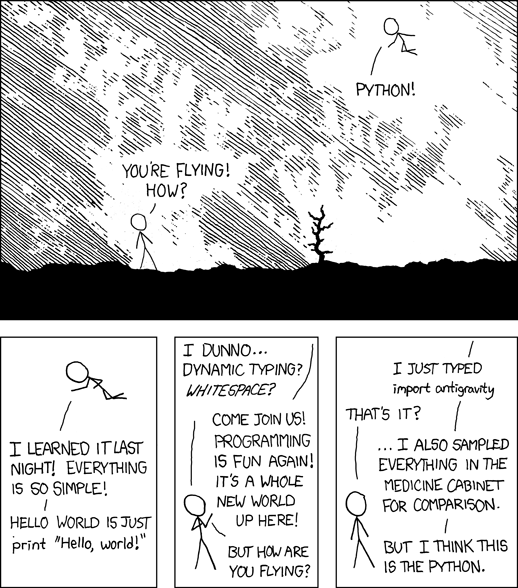
\includegraphics[height=8.5cm]{fig/xkcd.png}
\end{frame}

\begin{frame}\frametitle{Presentando Python}
	\begin{itemize}
		\item Dos versiones: 2.7 y \textbf{3.6}
		\item Libre, abierto y gratuito, con una comunidad enorme $\rightarrow$ todo a golpe de Google.
		\item Mil y una librerías abiertas y gratuitas.
		\item Rápido y fácil de escribir, puede ser lento de ejecutar.
	\end{itemize}
\end{frame}

\subsection{Librerías importantes}

\begin{frame}\frametitle{Librerías importantes}
	\begin{figure}
		\subfigure{
\includegraphics[height=1cm]{fig/numpy.png}}
		\subfigure{
\includegraphics[height=1cm]{fig/scipy.png}}
		\subfigure{
\includegraphics[height=1cm]{fig/matplotlib.png}}
		\subfigure{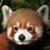
\includegraphics[height=1cm]{fig/pandas.jpg}}
		\subfigure{
\includegraphics[height=1cm]{fig/ipython.png}}
	\end{figure}

	\centering
	\textbf{Numpy}: cálculo numérico

	\textbf{Scipy}: cálculo científico

	\textbf{Matplotlib}: graficado
	
	\textbf{Pandas}: análisis de datos
	
	\textbf{IPython}: consola interactiva
\end{frame}

\subsection{Programación orientada a objetos}

\begin{frame}\frametitle{Programación orientada a objetos}
	Un \textbf{objeto} tiene \textbf{métodos} (``funciones'') y \textbf{atributos} (``variables'') que lo constituyen.

	\begin{itemize}
		\item \texttt{A.shape}
		\item \texttt{z.conjugate()}
		\item \texttt{v.reshape((3,4))}
	\end{itemize}

	Todo Python trabaja con objetos\footnote{\tiny (hasta donde yo sé)}
\end{frame}


\section{Sintaxis básica de Python}

\section{Numpy: el \texttt{ndarray}}

\section{Scipy}

\section{Matplotlib.pyplot}

\end{document}
